\chapter{Linux knowledge}

\section{Compilation}
 a compiler driver (that invokes the language preprocessor, compiler,
 assembler, and linker, as needed on behalf of the user) can generate three
 types of object files depending upon the options supplied to the compiler
 driver. Technically an object file is a sequence of bytes stored on disk in a
 file. These object files are as follows:
 \begin{itemize}
     \item   Relocatable object file: These are static library files. Static
         linkers such as the Unix ld program take collection of relocatable
         object files and command line arguments as input and generate a fully
         linked executable object file as output that can be loaded into memory
         and run. Relocatable object files contain binary code and data in a
         form that can be combined with other relocatable object files at
         compile time to create an executable object file.
     \item   Executable object file: These are executable files contain binary
         code and data in a form that can be copied directly into memory and
         executed.
     \item   Shared object file: These special type of relocatable object files
         are loaded into memory and linked dynamically, at either load time or
         run time.
 \end{itemize}

Object files have a specific format, however this format may vary from system
to system. Some most prevalent formats are \verb+.coff+ (Common Object File
Format), \verb+.pe+ (Portable Executable), and \verb+elf+ (Executable and
Linkable Format).

\section{Memory Layout of C Program}
 The actual layout of a program's in-memory image is left entirely up to the
 operating system, and often the program itself as well. This article focus on
 the concepts of code and data segments of a program and does not take any
 specific platform into account. For a running program both the machine
 instructions (program code) and data are stored in the same memory space. The
 memory is logically divided into text and data segments. Modern systems use a
 single text segment to store program instructions, but more than one segment
 for data, depending upon the storage class of the data being stored there.

 \begin{figure}
  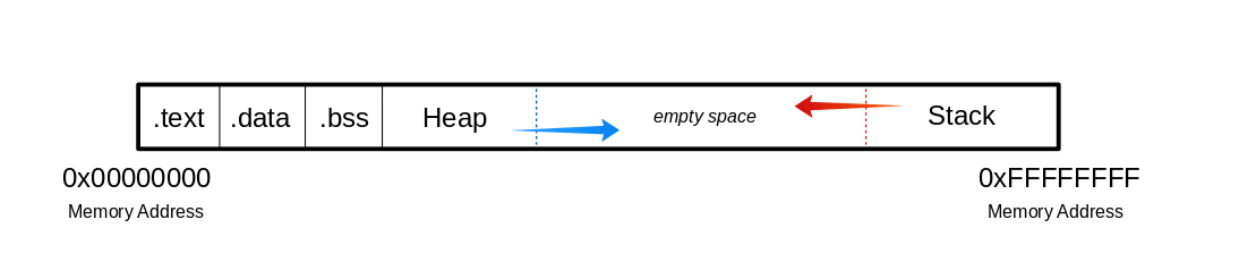
\includegraphics[width=\linewidth]{binary/linux_knowledge/images/memory-layout.png}
  \caption{Linux memory layout}
  \label{fig:linux-memory-layout}
\end{figure}

\subsection{Text Segment}

text segment contains machine code of the compiled
program. The text segment of an executable object file is often read-only
segment that prevents a program from being accidentally modified.

\subsection{Data Segments}

Data segment stores program data. This data could be in form of initialized or
uninitialized variables, and it could be local or global. Data segment is
further divided into four sub-data segments (initialized data segment,
uninitialized or \verb+.bss+ data segment, stack, and heap) to store variables
depending upon if they are local or global, and initialized or uninitialized.

\subsubsection{Initialized Data or Data Segment}

Initialized data or simply data segment stores all global, static, constant,
and external variables (declared with \verb+extern+ keyword) that are initialized
beforehand.

\subsubsection{Uninitialized Data or bss Segment}

Contrary to initialized data segment, uninitialized data or \verb+.bss+ segment stores
all uninitialized global, static, and external variables.This section occupies
no actual space in the object file; it is merely a place holder. Object file
formats distinguish between initialized and uninitialized variables for space
efficiency; uninitialized variables do not have to occupy any actual disk space
in the object file.

\subsubsection{Stack Segment}

Stack segment is used to store all local variables and is used for passing
arguments to the functions along with the return address of the instruction
which is to be executed after the function call is over. Local variables have a
scope to the block which they are defined in; they are created when control
enters into the block. Local variables do not appear in data or bss segment.
Also all recursive function calls are added to stack. Data is added or removed
in a last-in-first-out manner to stack. When a new stack frame needs to be
added (as a result of a newly called function), the stack grows downward.

\subsubsection{Heap Segment}
 Heap segment is also part of RAM where dynamically allocated variables are
 stored. 

The stack and heap are traditionally located at opposite ends of the process's
virtual address space.


\section{x86 function calling convention}

\subsection{Before call}
push arguments of the function (in reverse order)
\begin{verbatim}
0x08048420 <+37>: mov DWORD PTR [esp],eax
0x08048423 <+40>: call 0x80483e4 <add_numbers>
0x08048428 <+45>: mov DWORD PTR [esp+0x14],eax
\end{verbatim}

subsection{unction prologue}
\begin{itemize}
        \item Pushes current base pointer onto the stack, so it can be restored
            later.
        \item Value of base pointer is set to the address of stack pointer
            (which is pointed to the top of the stack) so that the base pointer
            will point to the top of the stack.
        \item Moves the stack pointer further by decreasing  its value, to make
            room for the function's local variables.
        \item Then, local variables of the function are pushed on the stack.
\end{itemize}

\begin{verbatim}
 0x080483e4 <+0>: push ebp
 0x080483e5 <+1>: mov ebp,esp
 0x080483e7 <+3>: sub esp,0x10
\end{verbatim}

\subsection{Function epilogue}
reverses the actions of the function  prologue and returns control to the
calling function

\begin{itemize}
        \item Drop the stack pointer to the current base pointer, so room
            reserved in the prologue for local variables is freed.a
        \item Pops the base pointer off the stack, so it is restored to its
            value before the prologue.
        \item Returns to the calling function, by popping the previous frame's
            program counter off the stack and jumping to it.
\end{itemize}

\begin{verbatim}
	mov	esp, ebp
	pop	ebp
	ret
# x86 processor contains a built-in instruction  equivalent to the above code:
0x080483f9 <+21>: leave
0x080483fa <+22>: ret
\end{verbatim}


